\chapter{Inertial Waves in a Rotating Cone}

\section{Introduction}

Following the introduction and validation of the immersed boundary methods for no-slip conditions,
we now want to exemplarly investigate a fluid system using these methods
and see if we can reproduce some of the expected physical properties.\\
In relation to the research focus of the geophysical fluid mechanics research group there are a variety
topics of interest.
One area of research lies in the exploration of dynamo effects in geological and stellar system.
In particular this means the generation of magnetic fields by electrically conducting fluids on large scales.
In this thesis we will not consider MHD-equations.
However in general it is considered that the helicity of a fluid, given by
\begin{align}
    v curl v
\end{align}
is directly linked to dynamo action [CITE].
Therefore, beside inertial wave propagation we want to observe a possible large helicity.
For the system we describe in the following section one further application
would be to study inertial wave excitaton by turbulence.

\section{Theoretical description}

The objective we have in mind is the numerical computation of inertial wave excitation inside a liberating cone.
The system was already investigated in an experimentally setup [CITE].
Here we want to give a brief overview of the theoretical properties and experimental results.\\
The schematic setup of the experiment is shown in figure ().
It contains of a cone given by the radius $R$ and the height $h$, resulting into an angle $\alpha = \tan()$.
The cone is rotating with a modulated frequency

\begin{figure}[!tbp]
  \centering
  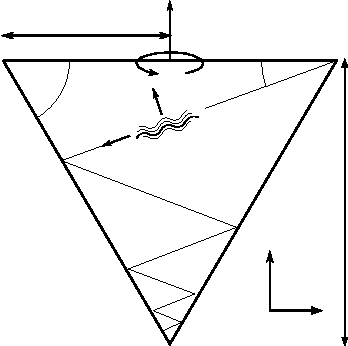
\includegraphics[width=0.5\textwidth]{gfx/cone/cone.pdf}\label{fig:cone_cone}
  \caption{blabla}
\end{figure}

\begin{align}
\Omega(t) = \Omega_0 + \epsilon \omega \cos(\omega t)
\end{align}

The modulation of the rotation frequency is also denoted as libration [RIGHT?] and can be used as a possible mechanism
for inertial wave exitation [CITE].
The overall idea of the setup is to introduce a geometry containing a singularity and study the influence on the ability of
the system to develop inertial eigenmodes.
Let us recall that the dispersion relation and group velocity of an inertial wave paket is given by

\begin{align}
    \omega = \frac{2\vec{\Omega}\vec{K}}{K} = 2 \Omega \cos\Theta ; \vec{c}_g = -\frac{2\vec{K}\times (\vec{\Omega} \times \vec{K})}{K^3}
\end{align}

with the wavenumber $\vec{K}$.
Let us now consider the propagation of an interial wave paket from the top edge of the cone as shown.
As discussed in section (), the reflection of inertial waves up on a  plane wall is a violation of snell's law.
For each reflection the propagation angle with respect to the rotation axis stays constant,
whereas the group velocity decreases.
It can be shown that for all path i.e. $L$ and $L^o$ the propagation time of the wave energy stays constant [CITE]
\begin{align}
    \frac{K^o}{K} = \frac{\cos(\Theta - \alpha)}{\cos(\Theta + \alpha)}
\end{align}
This means that the overall propagation time into the apex of the cone becomes infinity, along with the energy density and the wave number.
In conclusion it follows that since no reflection out of the cone apex can occur, the possibilty of inertial eigenmodes is not given.\\
In the experimental setup described by [] the experiment was compared to another setup where the cone was replaced with a frustum of a cone,
thus a bottom blade to enable the reflection of inertial waves was inserted.
As a result for the cone, a continuos wave spectrum could be observed in comparision to a discrete spectrum  for the frustum.\\

\section{Implementation}

For the numerical implementation of the experiment, we can now use a modified set of the equations
introduced in section (X.X).
For the setup we choose a modulated roation rate
\begin{align}
\Omega(t) = 1 + \epsilon \cos(\omega t)
\end{align}
for the non-dimensionalized system with $\vec{v}^* = bla$.



Since we now consider a time dependent rotation rate, there are two possibiliies.
First of all, we can consider a rotating coordinate system with a constant velocity $\Omega_0$.
This means the we can directly use the equations () to (), however since the overall rotation rate of the system is
modulated, it is necessary to introduce the boundary conditions

\begin{align}
    \vec{v}|_{Border}  = \Omega \times \vec{r} = \begin{bmatrix}
           -y \epsilon \cos(\omega t) \\
           -x \epsilon \cos(\omega t) \\
           0\\
         \end{bmatrix}
\end{align}

The alternative option is the introduction of a accelerated frame of reference.
In this case the boundary conditions do not need to be modified, but the coriolis forcing term is given by (CITE)

\begin{align}
    \vec{f} &= 2 \vec{\Omega} \times \vec{v} + \pdn[]{t}\left(\vec{\Omega} \times \vec{v} \right) \\
            &= \begin{bmatrix}\\
           -y \epsilon \cos(\omega t) \\
           -x \epsilon \cos(\omega t) \\
           0\\
         \end{bmatrix}
            &= \begin{bmatrix}\\
           -y \epsilon \cos(\omega t) \\
           -x \epsilon \cos(\omega t) \\
           0\\
         \end{bmatrix}
\end{align}

In the last step a linearization of the equation was performed.
Since we are in interested in the propagation of intertial modes this
step was performed to eleminate all possible non-linear effects which could occur.
Furthermore the non-linear advection term was removed from the equations.

\newpage

\section{Simulations}
\subsection{Liberating Cylinder}

Before the simulation of the cone we want to test the implementation of



As a first system we want to investigate the

- erstes test system cylinnder\\
- expectation

- verglein von den bedien implementierungen\\
- first test omega = 1.2 ...\\
- diskussion rand compare to tcflow \\
- test serie verschiede methoden\\
- spektrum dargesstel\\
- evtl raytracer  comparison
- heliziätte dargstellt\\
- results diskussion ip kaputt heli 0 etc \\

\subsection{Transition from Cylinder to Cone}

-description\\
-verfahren und serie\\
-diskussion oberer rand\\
-eigenschaften und influence oberer rand \\

\subsection{Cone}

-nun cone mit und ohne spitze
-teste den einfluss der oberen kante blablabla

-serien vergleich diskussion\
-helizität diskussion\\


In order to test



As a first test

\section{Numerical Viscosity}
